\documentclass[12pt]{extreport}
\usepackage[utf8]{inputenc}
\usepackage{geometry}
\usepackage{cancel}
\usepackage{graphicx}
\usepackage{amssymb}
\usepackage{float}
\graphicspath{ {images/} }
 \geometry{
 a4paper,
 total={170mm,257mm},
 left=20mm,
 top=20mm,
 }
\title{Project Report + User Manual}
\author{Kanak Agrawal 150050016 \\ Ajay Yadav 150050056 \\ Yash Wagh  150050023}
\date{November 5, 2016}



\begin{document}

\maketitle
  \chapter*{Overview}
This manual contains description on how to use the Feeder20 app designed by IITBombay students under Prof. Sharat Chandran as a course project. The App is meant for the students and help them in managing there tough schedule in colleges. For professores it provides them a platform to have regular feedback from students about the course.

  \chapter*{Django Web App}
  To use the app, have django installed on your laptop along with restframework. Go ahead and start the app by commands as mentioned in readme.txt. 
  
  \begin{itemize}
  \item There will be an admin with power to add courses and assign instructor to it. For assigning instructor, instructor should already be registered in the app.
  \item Admin also has to select a list of students to enroll for the course.(Presently in version 1.0, there is no featrue to enroll students to existing courses. Therefore make sure to enroll all students while adding course.)\\
  Whenever a course is add, 2 dates, midsem and endsem exam are also provided and corresponding exam and feedback deadlines are initialized at that time
  \begin{figure}[ht!]
    \centering
    \begin{minipage}{.5\textwidth}
      \centering
      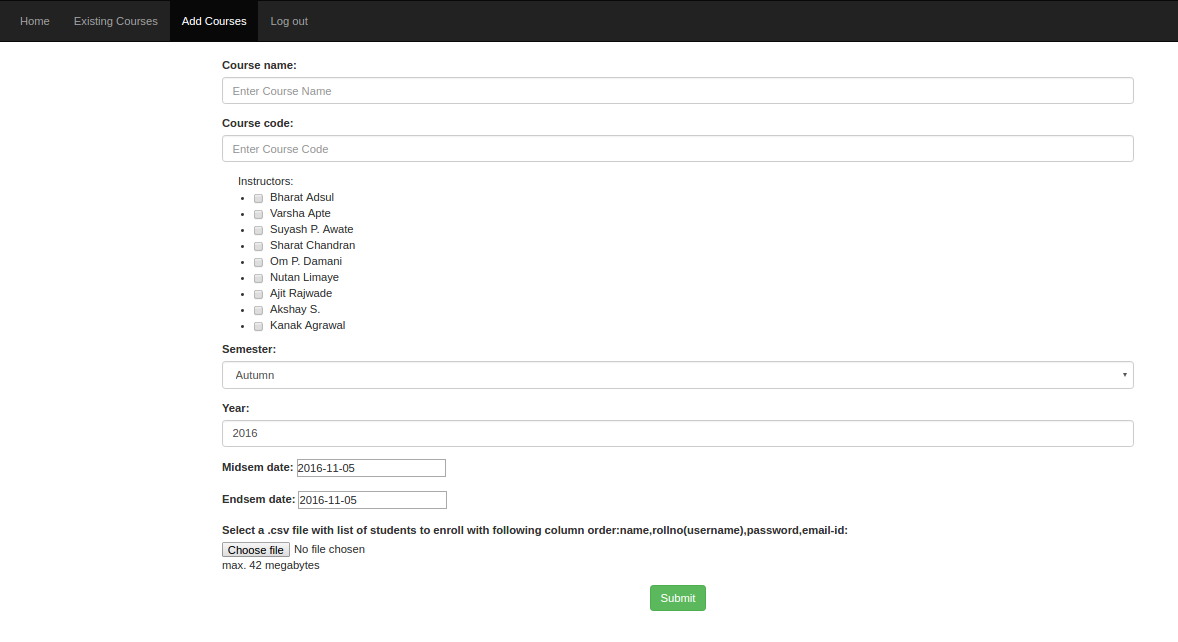
\includegraphics[width=.4\linewidth]{images/admin_addcourses.png}
      \caption{Add courses \label{overflow}}
      \label{fig:sub1}
    \end{minipage}%
    \begin{minipage}{.5\textwidth}
      \centering
      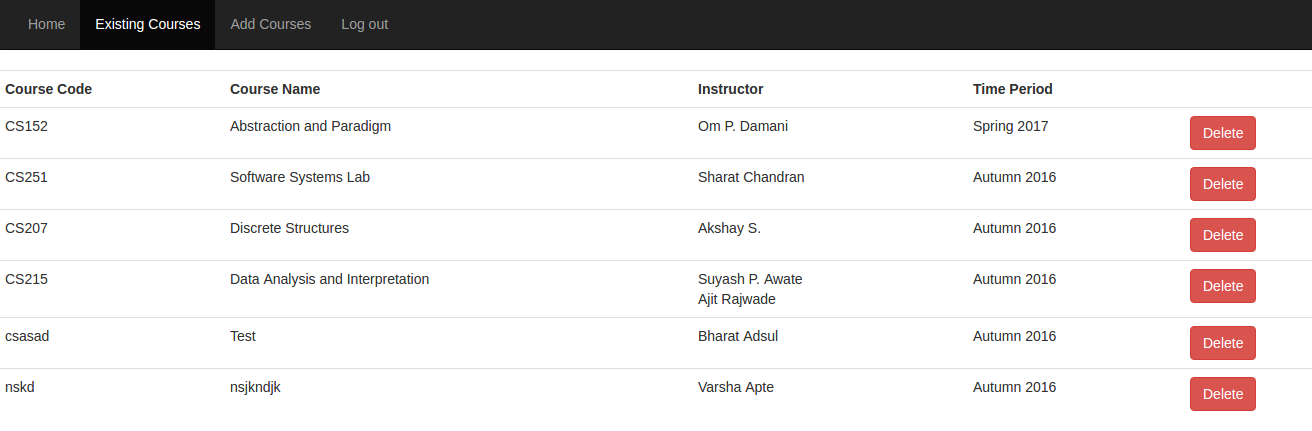
\includegraphics[width=.4\linewidth]{images/admin_courses.png}
      \caption{View courses \label{overflow}}
      \label{fig:sub1}
    \end{minipage}%
  \end{figure}
  \item Instructor can registor or have google or Facbook sign in. (The uniqueness of an account is determined by the email id and hence if instructor logs in by facebook once and google next time and have different email ids in the two, then he will end up having 2 different sign in in the app which won't be synced with each other.)
  \begin{figure}[ht!]
    \centering
    \begin{minipage}{.5\textwidth}
      \centering
      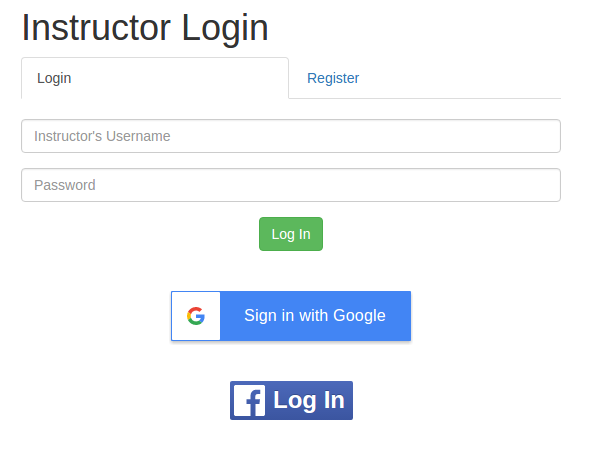
\includegraphics[width=.4\linewidth]{images/instructor_login.png}
      \caption{Instructor Login \label{overflow}}
      \label{fig:sub1}
    \end{minipage}%
    \begin{minipage}{.5\textwidth}
      \centering
      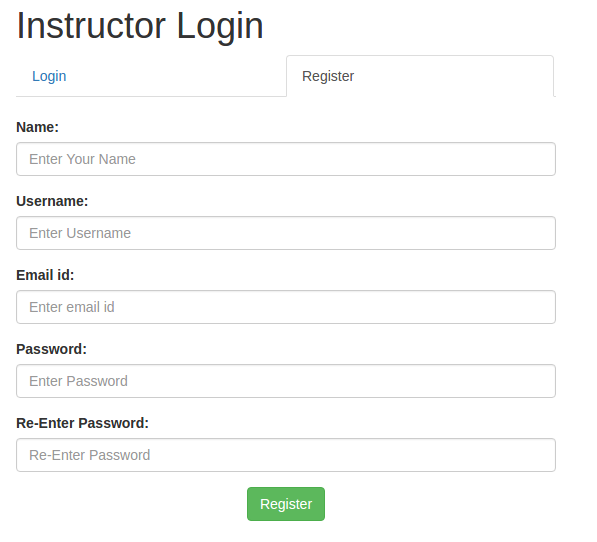
\includegraphics[width=.4\linewidth]{images/instructor_register.png}
      \caption{Instructor Register \label{overflow}}
      \label{fig:sub1}
    \end{minipage}%
  \end{figure}
  \item Now the instructor can move to different tabs and add or view feedback and assignment deadlines for the courses he/she is teaching.
  \item Add Feedback: For any feedback, instructor has 2 types of question to ask, rating question whose answer will be a rating between 1 to 5 and a subjective question whose answer will be at most of 300 letters. The cool feature about this is that he/she can add any number of questions dynamically.(Note: Make sure you fill the nn-question fields in proper format, else on submit all the filled questions will get clear and you will be asked again to fill them.)
  \item Add  Deadline: Its plain and simple just fill date, time, name and course.
  \begin{figure}[ht!]
    \centering
    \begin{minipage}{.5\textwidth}
      \centering
      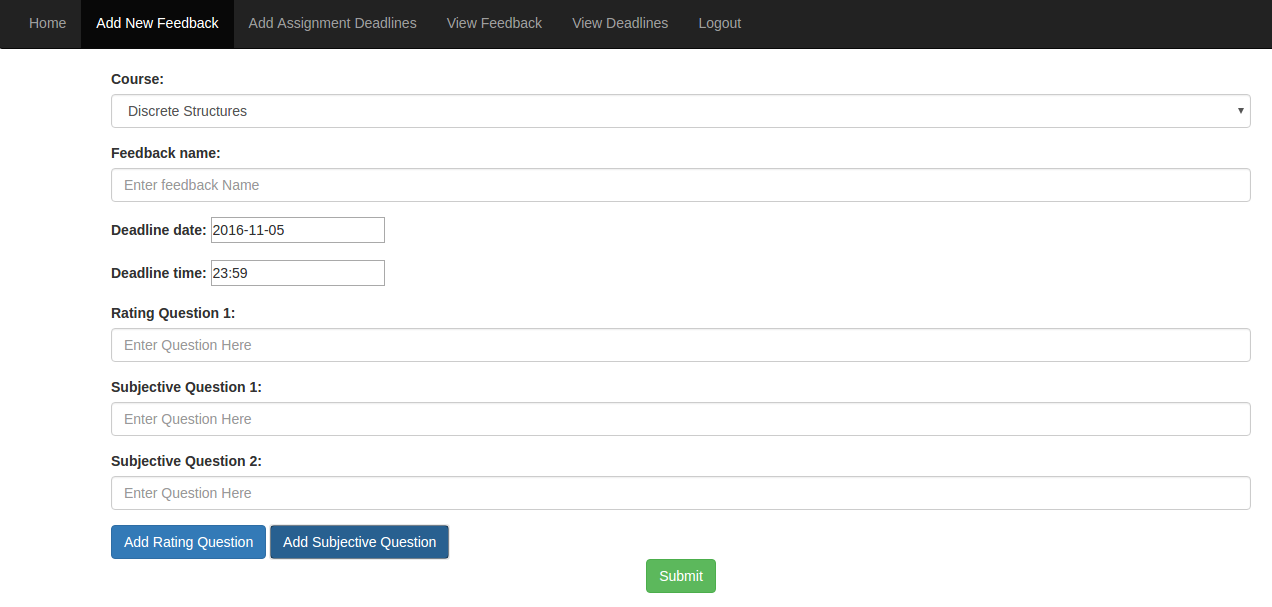
\includegraphics[width=.4\linewidth]{images/instructor_addfeedback.png}
      \caption{Add Feedback \label{overflow}}
      \label{fig:sub1}
    \end{minipage}%
    \begin{minipage}{.5\textwidth}
      \centering
      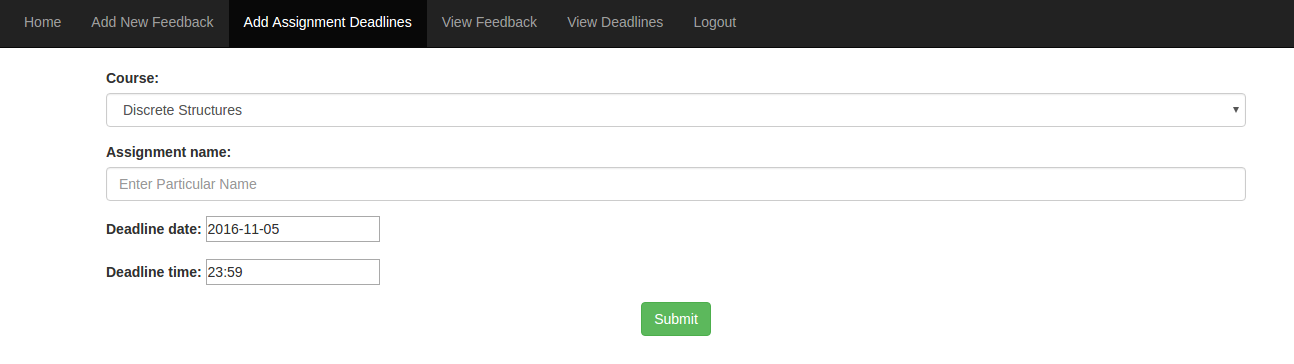
\includegraphics[width=.4\linewidth]{images/instructor_addDeadline.png}
      \caption{Add Deadline \label{overflow}}
      \label{fig:sub1}
    \end{minipage}%
  \end{figure}
  \item view Feedback: This is the feature which makes this app a must for college. It provides instructor with cool graphs of feedback of rating question and helo them make changes accordingly in the course. Also, for subjective questions instructor get all the answers for a question in a fix height with scrolling option making it good to use.
  \begin{figure}[ht!]
    \centering
    \begin{minipage}{.5\textwidth}
      \centering
      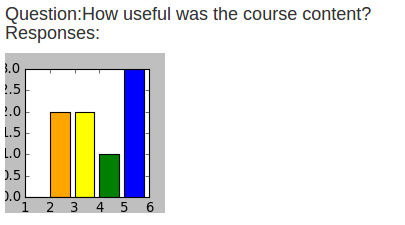
\includegraphics[width=.4\linewidth]{images/ratingAnswer.png}
      \caption{Rating feedback with bar graph\label{overflow}}
      \label{fig:sub1}
    \end{minipage}%
    \begin{minipage}{.5\textwidth}
      \centering
      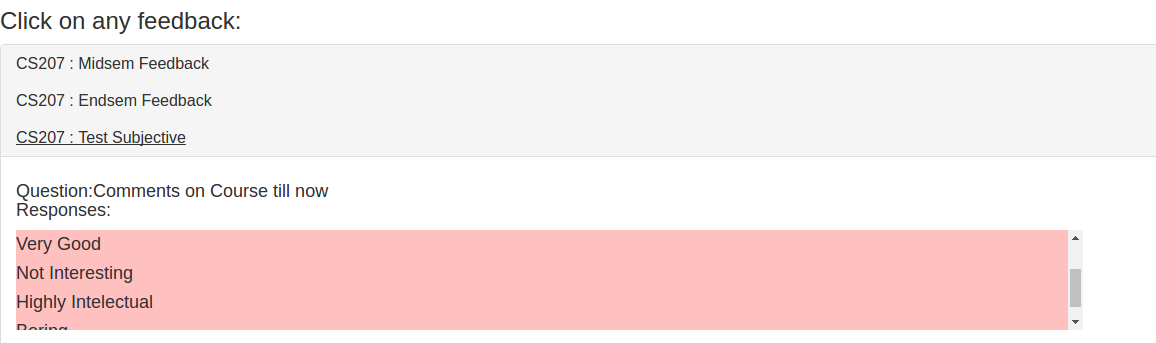
\includegraphics[width=.4\linewidth]{images/subjectiveAnswers.png}
      \caption{Subjective Answers with scroller \label{overflow}}
      \label{fig:sub1}
    \end{minipage}%
  \end{figure}
  \item view Deadline: This feature in the app distinguishs between deadlines completed and deadline due. Also you can navigate between assignment deadlines and feedback deadlines. Don't worry that there is no edit deadline option. For now you can use delete deadline and add again with changes.
  \begin{figure}[ht!]
    \centering
      \centering
      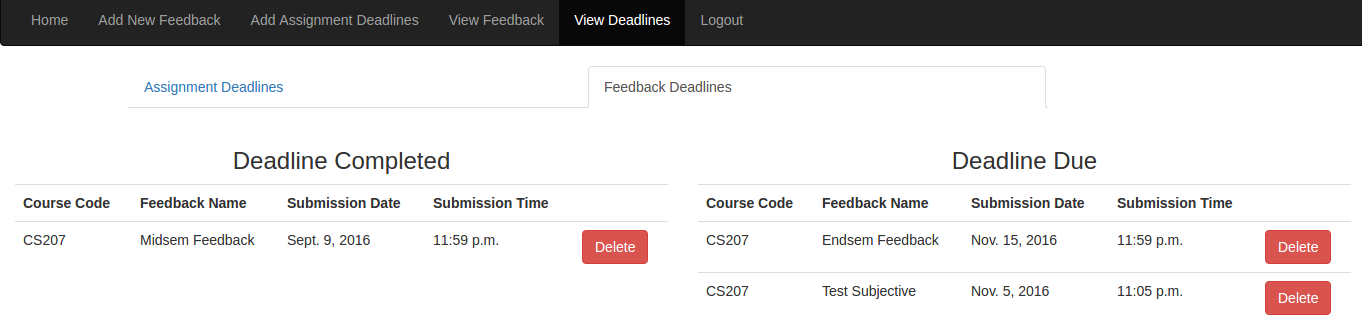
\includegraphics[width=.4\linewidth]{images/viewDeadline.png}
      \caption{view Dealine\label{overflow}}
      \label{fig:sub1}
  \end{figure}
  \item Note: Make sure to logout from the app else, it would get loggedin automatically next time.

  \end{itemize}

  \chapter*{Android App}
  To use the app, have android studion installed on your laptop and open the project. Now run it on an emulator.
  
  \begin{itemize}
  \item The first Activity is the login activity which ask for username(roll number) and password provided by admin to all students. If invalid credentials are entered it tells "Invalid Credential". Else you can log in.
  \begin{figure}[ht!]
    \centering
    \begin{minipage}{.5\textwidth}
      \centering
      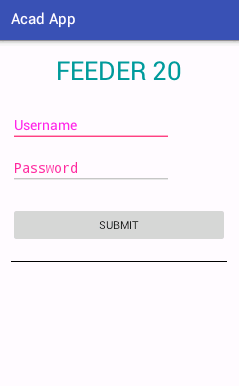
\includegraphics[width=.4\linewidth]{images/appLogin.png}
      \caption{Login\label{overflow}}
      % \label{fig:sub1}
    \end{minipage}%
    \begin{minipage}{.5\textwidth}
      \centering
      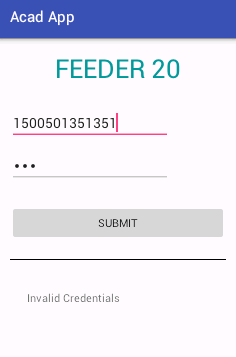
\includegraphics[width=.4\linewidth]{images/appinvalidLogin.png}
      \caption{Login \label{overflow}}
      % \label{fig:sub1}
    \end{minipage}%
  \end{figure}
  \item Once logged is student he remains logged in untils he logs out. 
  \item He/she can see all deadlines in calendar view. On selecting any date. The dates are coured as per different courses. If a date has more than one course deadline, then you will see only one of the colours but on clicking it you will see all the deadlines in respective colors.
  \begin{figure}[ht!]
    \centering
    \begin{minipage}{.3\textwidth}
      \centering
      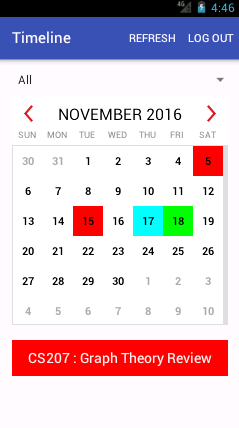
\includegraphics[width=.3\linewidth]{images/calendar.png}
      \caption{Only feedback\label{overflow}}
      % \label{fig:sub1}
    \end{minipage}%
    \begin{minipage}{.3\textwidth}
      \centering
      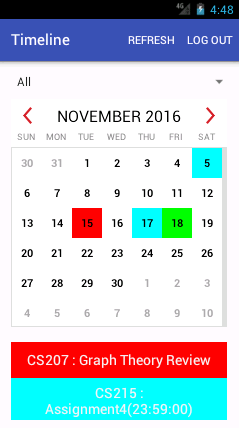
\includegraphics[width=.3\linewidth]{images/calendarMix.png}
      \caption{Mix courses\label{overflow}}
      % \label{fig:sub1}
    \end{minipage}%
    \begin{minipage}{.3\textwidth}
      \centering
      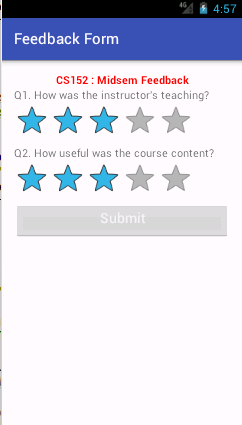
\includegraphics[width=.3\linewidth]{images/feedbackForm.png}
      \caption{Feedback Form\label{overflow}}
      % \label{fig:sub1}
    \end{minipage}%
  \end{figure}
  \item In case of feedback on selecting the feedback, user is directed to a new activity with feedback form. If feedback is already being filled then user is not allowed to fill again.
  \item For deadline, since there is no other data to show, it only display thename along with deadline time in bracket.
  \item There is feature to refresh and logout in the calendar activity.
  \item Also whenever the app, starts it automatically refreshes.
  \end{itemize}

  \chapter*{Reflection Essay}
The project as whole was a great great learning experience. Though a lot of time was invested in it, it never felt boring. Let us go point by point:
  \begin{itemize}
  \item The application of previous labs quite a lot, especially lab2, lab4 and lab9.(Also lab6 while typing this latex document :P)
  \item We used javascript in adding questions onclick in add feedback learnt in lab2. Also used accordion in view feedback.
  \item matplotlib was used for drawing bar graph.
  \item Apart from all this using already built frameworks(like rest-framework) to make thing pretty easier was a learning point on how to use others already written code.
  \item There was a point when we have to change a lot of our model because we didn't think through on how to send data in android app and all. This reminded us Linus Torvalds quote - "Bad programmers worry about the code. Good programmers worry about data structures and their relationships."
  
  \end{itemize}

\end{document}